%!TEX root = ../document.tex
\section{Implementation Ideas} \label{sec:IMPLEMENTATION_IDEAS}
%Lauritz
Besides providing an unobstrusive user interface, either implemented as a plugin for an existing integrated development environment or else in form of a complete development environment, an implementation of our idea would primarily require components that gather data contexts from actual program runs as well as components that support developers in selecting appropriate and interesting data contexts during development.

\subsection{Gathering Data Contexts}
As described in Section~\ref{sec:PAPER_PROTOTYPE} and \ref{sec:FINAL_PROTOTYPE}, our envisioned environment always presents relevant runtime data when developers interact with statements as, for example, when they click or hover on single lines of source code.
Further, developers should be able to evaluate arbitrary lines, including lines containing database queries, to see and understand the effects of their code on the application as well as the database layer.
That is, our approach relies on providing developers with actual runtime data and real database tables already during development and, therefore, depends on the availability of such data contexts for the presented code base.
Such data contexts need to be completely realistic and immediately available to be useful to developers.
Given these requirements, two approaches could provide data contexts for specific code sections of interest to the developer:
Either, the interactions with particular statements in code trigger deterministic test runs that cover that section or else, tracing the application's execution records data contexts in advance.
Recording data beforehand obviously also could rely on test runs, but could also be captured in deployed systems used by actual customer to provide evee more realistic runtime data.
Further, recorded data contexts need just be fetched from a database, which also could be an in-memory database, and, thus, potentially provides data contexts faster than establishing runtime data through running tests.
The time required to run tests depends on the granularity of the covering tests with a full spectrum from fine-grained, isolated unit tests to high-level, long-running acceptance tests.
However, running tests to emulate runtime during development would only require to store associations between code and tests, while recording in advance implies storing as much data as necessary to actually run any statements in the sources of an application.
A reasonable trade-off between space and time consumption, which we would probably investigate first, could record data not on the level of single statements but on the level of method scopes, when we assume deterministic code execution.
Such an implementation would record all data necessary to actually run a method with all its statement, including provided parameters, accessible state, and the the database at the moment the method is entered, as shown in Figure~\ref{fig:context_recording}.

\begin{figure}
    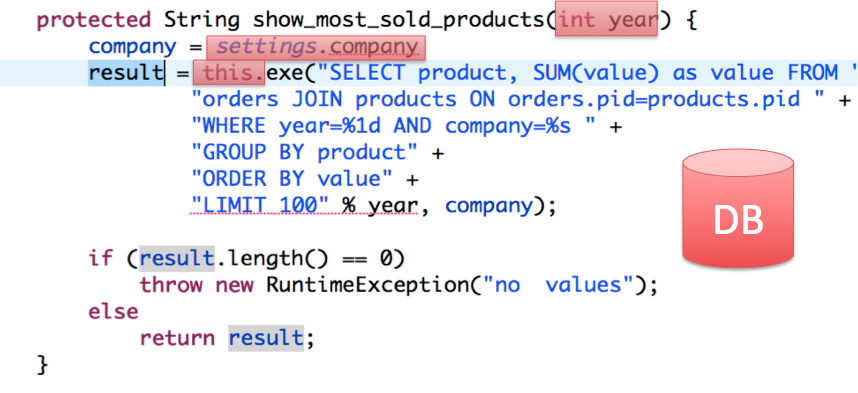
\includegraphics[width=\linewidth]{images/context_recording}
    \caption{Running the statements of this Java method with its embedded SQL query requires all data highlighted in red: the parameter, accessible state, and a database.}
    \label{fig:context_recording}
\end{figure}.

When a developer then interacts with a specific line in the method's body, we could use ordinary breakpoints to establish the necessary runtime data for that specific line of interest. 
Accessible state includes global state and depending on the used programming language also state from surrounding scopes as, for example, from surrounding functions or the receiver.
Snapshots of the database are necessary as methods that embedd queries might modify the database, potentially impeding subsequent runs of that method during the interactive development.
\subsection{Selecting Data Contexts}
The presented tracing approach generates potentially numerous data contexts for each method.
Given our tool traces actually live systems deployed at customers, each user interaction might lead to recorded data contexts for all method executions that such interactions trigger.
Further, even when our tool only traces test execution once on replicated databases, particular method might not only be executed in multiple test cases, but also multiple times in single test cases as, for example, obviously the case with methods called from loop bodies.
For these reasons, developers using our proposed environment might be confronted with many data contexts for each statement of interest.
However, as the number of available data contexts might be arbitrarily high and data context from the same trace might also overlap considerably, presenting all data contexts to the developer probably reduces usability significantly.
Approaches addressing this issue include automatic selection of interesting samples after clustering all data contexts, preselection of interesting data contexts through expert users, and combinations of those two methods.
Clustering data contexts could be based on several dimensions, including:
\begin{itemize}
  \item size of the associated database snapshot
  \item control flow that lead to this context
  \item execution time leading to the context
\end{itemize}
Nevertheless, even aided through automatic clustering or manual preselections, our tools should probably also support developers in exploring the full extent of available contexts and make the final decision on which specific data context they want to use during development.